\section{Introducción}
\subsection{Sistemas de Telecomunicación}
\begin{itemize}
\item\textbf{\Gls{teleco}:} Comunicación (intercambio de información) a distancia.
\item\textbf{\Gls{Sistema}:} Conjunto de medios y de métodos para el logro de un fin común.
\item\textbf{\Gls{Red}:} Conjunto organizado de recursos tanto físicos como lógicos que permiten la telecomunicación. La \gls{Red} es un recurso escaso que debe compartirse. Para esto se aplican técnicas de acceso múltiple y de multiplexación en las redes.
\item\textbf{\Gls{Servicio}:} Conjunto de medios físicos y lógicos operados y gestionados por un proveedor del \gls{Servicio}, que se ponen a disposición de un cliente, junto con unas normas de acceso y utilización, para satisfacer sus necesidades en materia de Telecomunicaciones.
\end{itemize}
\subsubsection{Clasificación de Servicios}
Los servicios se pueden clasificar atendiendo a los siguientes criterios:
\begin{itemize}
\item Básicos y suplementarios: Los servicios básicos son los que existen por sí mismos, como por ejemplo el servicio telefónico básico, en cambio los suplementarios existen asociados a algún servicio básico, como por ejemplo la identificación de llamada.
\item Clasificación \acrshort{ITU}-CCITT: Los servicios portadores son los que transportan la información. Los serviciosfinales o teleservicios incluyen ya el terminal final para poder ofrecer una comunicación completa o añaden capacidades suplementarias como de almacenamiento.
\item Colectivo de usuarios:intercomunicación, comunicación social; comercial, residencial.
\item Capacidad: Banda ancha o estrecha.
\item Modo de efectuar la comunicación: consulta, difusión,conversación, mensajería; simétricos, asimétricos.
\item Movilidad del usuario: movil, portátil, fijo.
\item Tipo de red: \acrshort{RTPC}, \acrshort{RDSI}, Radiodifusión.
\end{itemize}
\subsubsection{Principales servicios}
\begin{itemize}
	\item Servicio Telefónico: Servicio de comunicación por voz entre usuarios. Es un servicio de gran extensión en el cual se han introducido gran cantidad de avances como la digitalización o la movilidad.
	\item Servicio de transmisión de datos: Servicio de intercambio de información de naturaleza digital que se apoya o en la red telefónica o en la red de datos.
	\item Servicios de valor añadido: Servicios como el fax, el teletexto o el datáfono.
	\item Servicios de radiocomunicación: Servicios caracterizados por la inexistencia de un medio físico de enlace, lo que le permite ser movil y dar acceso a grandes públicos.
\end{itemize}
\subsubsection{Arquitectura de un sistema de Telecomunicación}
En la figura a continuación se pueden ver diferentes entidades funcionales y puntos de referencia (interfaces), interconexiones entre entidades funcionales. Las entidades funcionales son el conjunto de funciones en la red con una finalidad común que pueden comprender uno o varios dispositivos físicos, como los terminales, la red de transporte o la terminación de red. Los puntos de referencia (interfaces) son interconexiones entre entidades, en la figura se ven las interfaces U y S.
\begin{figure}[H]
\centering
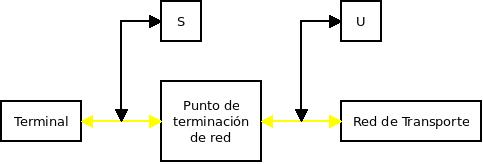
\includegraphics[width=\textwidth]{Imagen/arquisistemateleco.jpg}
\caption{Arquitectura básica de un sistema de Telecomunicación}
\label{}
\end{figure}
\subsection{Organismos reguladores de las Telecomunicaciones}
\begin{itemize}
	\item UIT (\acrshort{ITU}) Unión Internacional de Telecomunicaciones. Tienen la función de armonizar las telecomunicaciones a nivel global y para esto realizan estudios y formulan recomendaciones. Tiene varios organos permanentes
	\begin{itemize}
		\item Secretaría.
		\item UIT-R: Radiocomunicaciones (antiguo CCIR)
		\item UIT-T: Telegrafía, Telefonía y telemática (antiguo CCITT)
		\item Junta de registro de frecuencias
	\end{itemize}
	\item \acrshort{ISO} Organización Internacional de Estandarización. En españa está representada por la Agencia española de Normalización y Certificación. Esta se encarga de la elaboración de normas. Por ejemplo la ISO 9000 se ocupa de la gestión de la calidad.
	\item \acrshort{CEPT} Conferencia Europea de Administraciones de Correos y Telecomunicaciones. Su función es la armonizaciónde las telecomunicaciones a nivel europeo, proporcionando un foro de discusión para el fomento de las relaciones entre organismos reguladores europeos. 
	\item \acrshort{ETSI} European Telecommunication Standards Institute. Fue creado por el CEPT para la elaboración de normas y estandares sobre redes y sistemas.
	\item Dirección General para la Sociedad de la Información de la Comisión Europea. Políticas proyectos y programas relacionados con las tecnologías de la información.
	\item \acrshort{IEEE} Institute of Electrical and Electronic Engineers. Crea normas de efecto global.
	\item \acrshort{WARC} World Administrative Radio Conference. Define que bandas de frecunecia son de uso preferente a servicios concretos (antes eran dedicadas, ahora no).
	\item \acrshort{CNAF} Cuadro Nacional de Atribución de Frecuencias. Es la WARC de españa. Tanto este como el anterior tienen los siguientes roles:
	\begin{itemize}
		\item Atribución (de una banda de frecuencias): inscripción en el cuadro de atribución de bandas de frecuencias, de una banda de frecuencias determinada, para que sea utilizada por uno o varios servicios de radiocomunicación terrenal o espacial o por el servicio de radioastronomía en condiciones específicas. 
		\item Adjudicación (de una frecuencia o de un canal radioeléctrico): inscripción de un canal determinado en un plan, adoptado por una conferencia competente, para ser utilizado por una o varias administraciones para un servicio de radiocomunicación terrenal o espacial en uno o varios países o zonas geográficas determinados y según condiciones específicas.
		\item Asignación (de una frecuencia o de un canal radioeléctrico): autorización que da una administración para que una estación radioeléctrica utilice una frecuencia o un canal radioeléctrico determinado en condiciones específicas. 
	\end{itemize}
\end{itemize}
\subsection{Legislación de Telecomunicaciones}
\subsubsection{Ley 32/2003 de Noviembre}
Deroga la Ley General de Telecomunicaciones 11/1998 de 24 de Abril con el objetivo de liberalizar la competencia en Telecomunicaciones mediante el establecimiento de licencias para prestación de servicios de Telecomunicaciones. También incorpora la evolución de las Telecomunicaciones desde la liberalización, siguiendo las Directivas de la UE.
\subsubsection{Ley 9/2014}
El objetivo es mejorar la libre competencia y facilitar la inversión. Las principales diferencias son la inclusión de medidas estructurales para:
\begin{itemize}
	\item Facilitar el despliegue de nuevas redes (incluyendo expropiación de azoteas)
	\item Mejora de los servicios innovadores para los ciudadanos y abaratamiento de los mismos
\end{itemize}
Además se crea nueva comisión interministerial de \acrshort{RF} y Salud. Se lucha por la simplificación del despliegue de redes (algunas medidas muy controvertidas). Otro objetivo es garantizar que en 2017, el 100\% de los hogares tengan un ancho de banda de 10Mbps y en 2020, a 30MBps (100\%) y más de 100Mbps (50\%).